\documentclass[11pt]{bxart}
\usepackage[utf8]{inputenc}
\usepackage[widespace]{fourier}
\usepackage{microtype}
\usepackage{graphicx}
\usepackage{wrapfig}

% list only sections for the table of contents
\setcounter{tocdepth}{1}

\title{\textbf{Raising a God}}
\author{Alex Schröder}

\begin{document}

\begin{titlepage}
  \maketitle
  \centering
  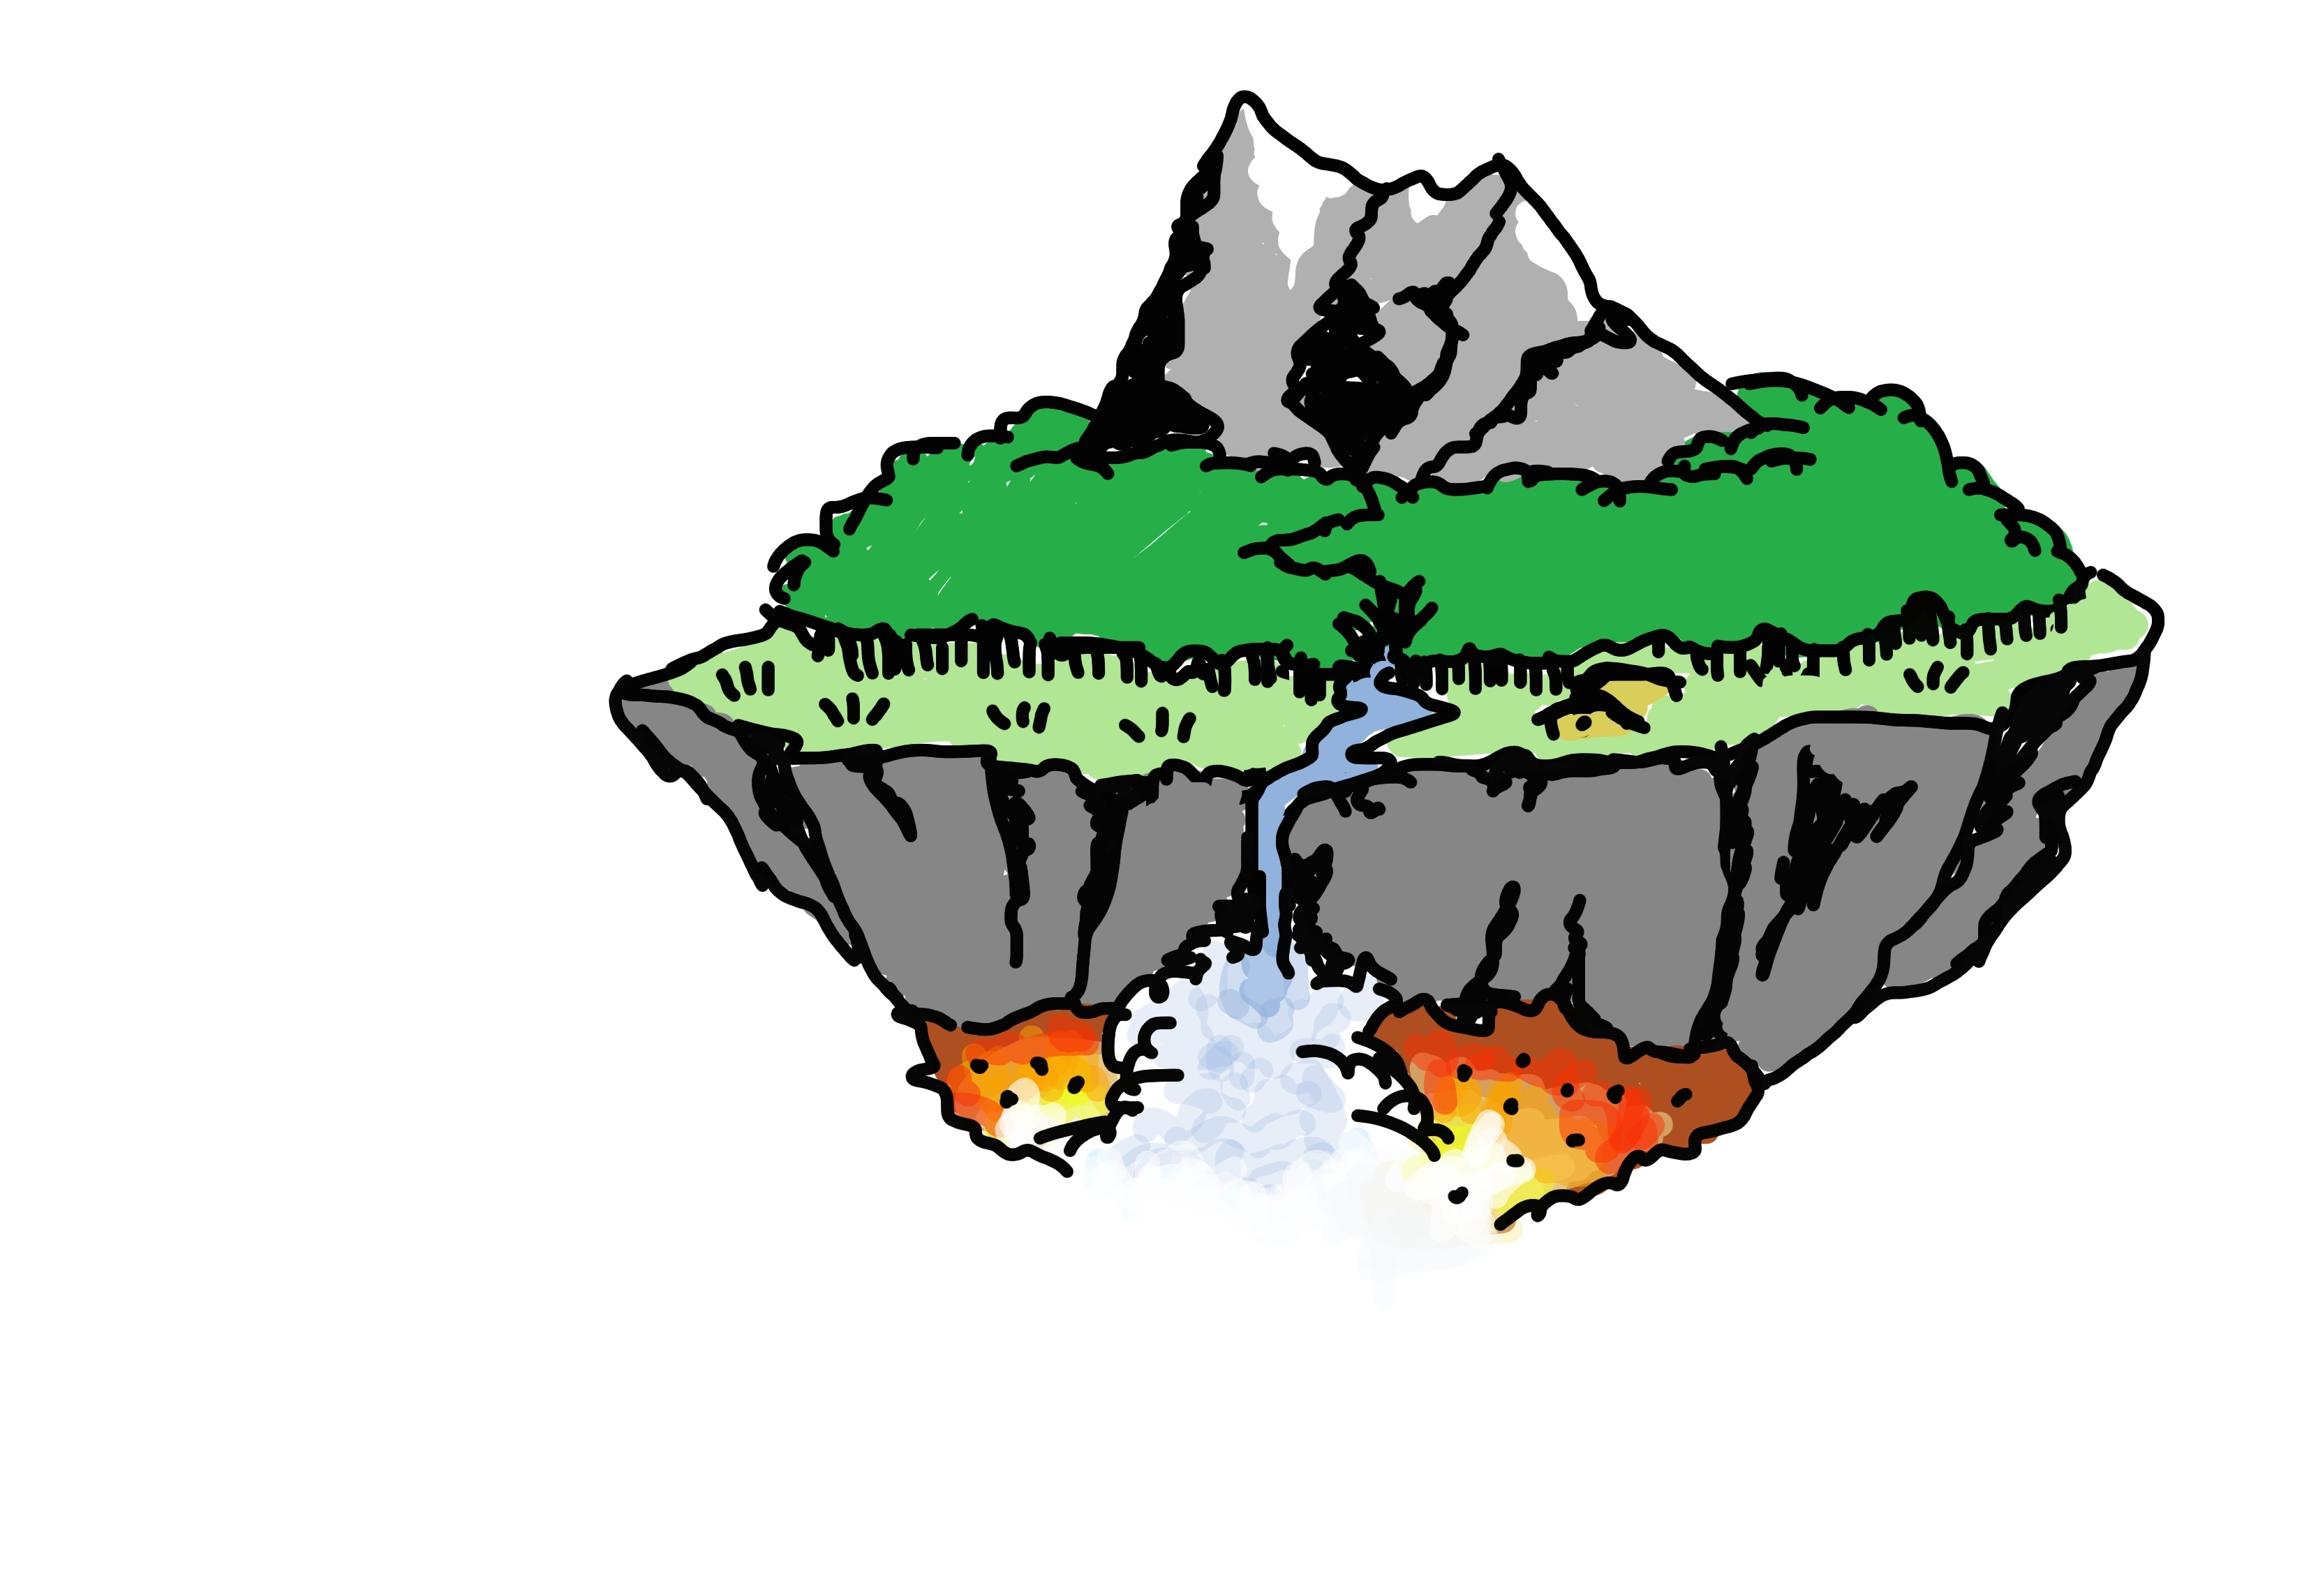
\includegraphics[width=10cm]{Floating-Island.jpg}
  \tableofcontents
\end{titlepage} 

\section{Introduction}

This is a mini-campaign for players in their mid levels, levels five to ten. Player characters start looking for a place to build their castles and tower, thieves look to expand their network of spies and thieves, clerics start meddling in the affairs of the gods.

Here are some of long term goals for your players:

\begin{itemize}
\item End the slave trade on Hinia Oot
\item Raise the dead god of light, Arden
\item Topple the reign of the grey elf witch Susrael
\item Prevent the rise of the demon lord Tsathoggua
\end{itemize}

\section{Gods}

There is a chance that the gods will send one of their agents to help if their name is called. In order to succeed, players need to keep track of \textbf{a score for each god} they care about. As characters do things to honor or spite the various gods, their score goes up. This could be about saving or killing their followers, building altars and temple in their name, defiling their altars or acting on visions sent by them. This score is the percent chance that the god will act when their name is called. Whether the agents appearing will in fact help the characters depends on their past actions. An evil demon lord like Set might still send a naga to help a paladin of Mitra, hoping to mess with them.

When paladins and clerics cast \textbf{spells of level four and higher}, the spell effect usually involves the appearance of such an agent, and an opportunity for some discourse.

\textbf{Freya} is the goddess of winter, of spring, of fertility, of grain, of war, of cats and boars, of magic. She leads the valkyries and collects half the slain in battle. These dine with her in Sessrúmnir, her hall in Asgard.

\textbf{Odin} is the god of wisdom, of magic and poetry, of war, of eagles and ravens, of runes, of wanderers. He wields a magic spear, he raises the dead, he rides an eight legged horse called Draupnir. The other half of the slain in battle dine with him in Valhalla, his hall in Asgard.

In times of need, both of them will send a \textbf{valkyrie} named \textit{War}, \textit{Mercy} \textit{Spear}, \textit{Cruel} or \textit{Fight}: HD 6 AC 2 1d8 \textit{sword+3} MV 18 ML 12 XP 820, flying, only harmed by magic or magic weapons. The swords of valkyries are bright swords of light. When swinging such a sword, the wielder is compelled to shout for blood and glory at the top of their voice. Also, when allies are fighting, the owner of such a sword is compelled to draw it and join this melee. When resisting such a compell for the third time, the sword looses its magic. The owner is considered unfit to wield it.

\textbf{Loki} is the god of lies, of deceit, of misdeeds, of excuses and explanations, of looking the other way, of tricksters, thieves and shape changers, a friend of giants, the innocently accused, the misunderstood and the innocent.

In times of need, he might send a nameless \textbf{shape changer}: HD 4 AC 5 1d12 MV 9 ML 10 XP 190, \textit{polymorph} at will, immune to \textit{sleep} and \textit{charms}. Clearly, mostly useful when in need of deception.

\textbf{Mitra} is the goddess of law, of fire, of bulls, of contracts, of bonds, the swearing of oaths, of honesty and truth, of loyalty and sacrifice for the community. 

In times of need, she might send a \textbf{minotaur} named \textit{Silence}, \textit{Calm}, \textit{Truth Teller} or \textit{Spirit Guide}: HD 6 AC 6 1d6/1d6 MV 12 ML 12 XP 820, \textit{mesmerize} any listeners at will (listeners must save vs. spells or stop hostilities speak nothing but the truth), immune to \textit{sleep} and \textit{charms}.

\textbf{Set} is the demon lord of snakes and crocodiles, of assassins, of revenge, of spies and diplomats, of poison makers, of death traps, of hypnotists and mind benders.

In times of need he will send a \textbf{naga} named \textit{Sweet Stab}, \textit{Revenge}, \textit{Crocodile Tears} or \textit{Coral Death}: HD 9 AC 7 1d8 \textit{poison} MV 6 ML 12 XP 2400, \textit{fireball} (7d6) 3/day, \textit{charm person} at will, only harmed by magic or magic weapons.

\textbf{Pazuzu} is the demon lord of pestilence, of miscarriage, of famine and disease, of crows and vultures, of temptation and betrayal.

In times of need he will send a \textbf{vulture demon} named \textit{Gangrene}, \textit{Pestilence}, \textit{Corpse Eater} or \textit{Baby Killer}: HD 8+1 AC 5 1d4/1d4/1d6/1d6/1d8 MV 18 ML 11 XP 2420, flying, only harmed by magic or magic weapons.

\section{Astral Sea}

The Astral Sea is an air filled plane, black and silent. It can be sailed by flying ships. There are many \textit{gates} in the Astral Sea, connecting it to many other planes.

\begin{figure*}
  \centering
  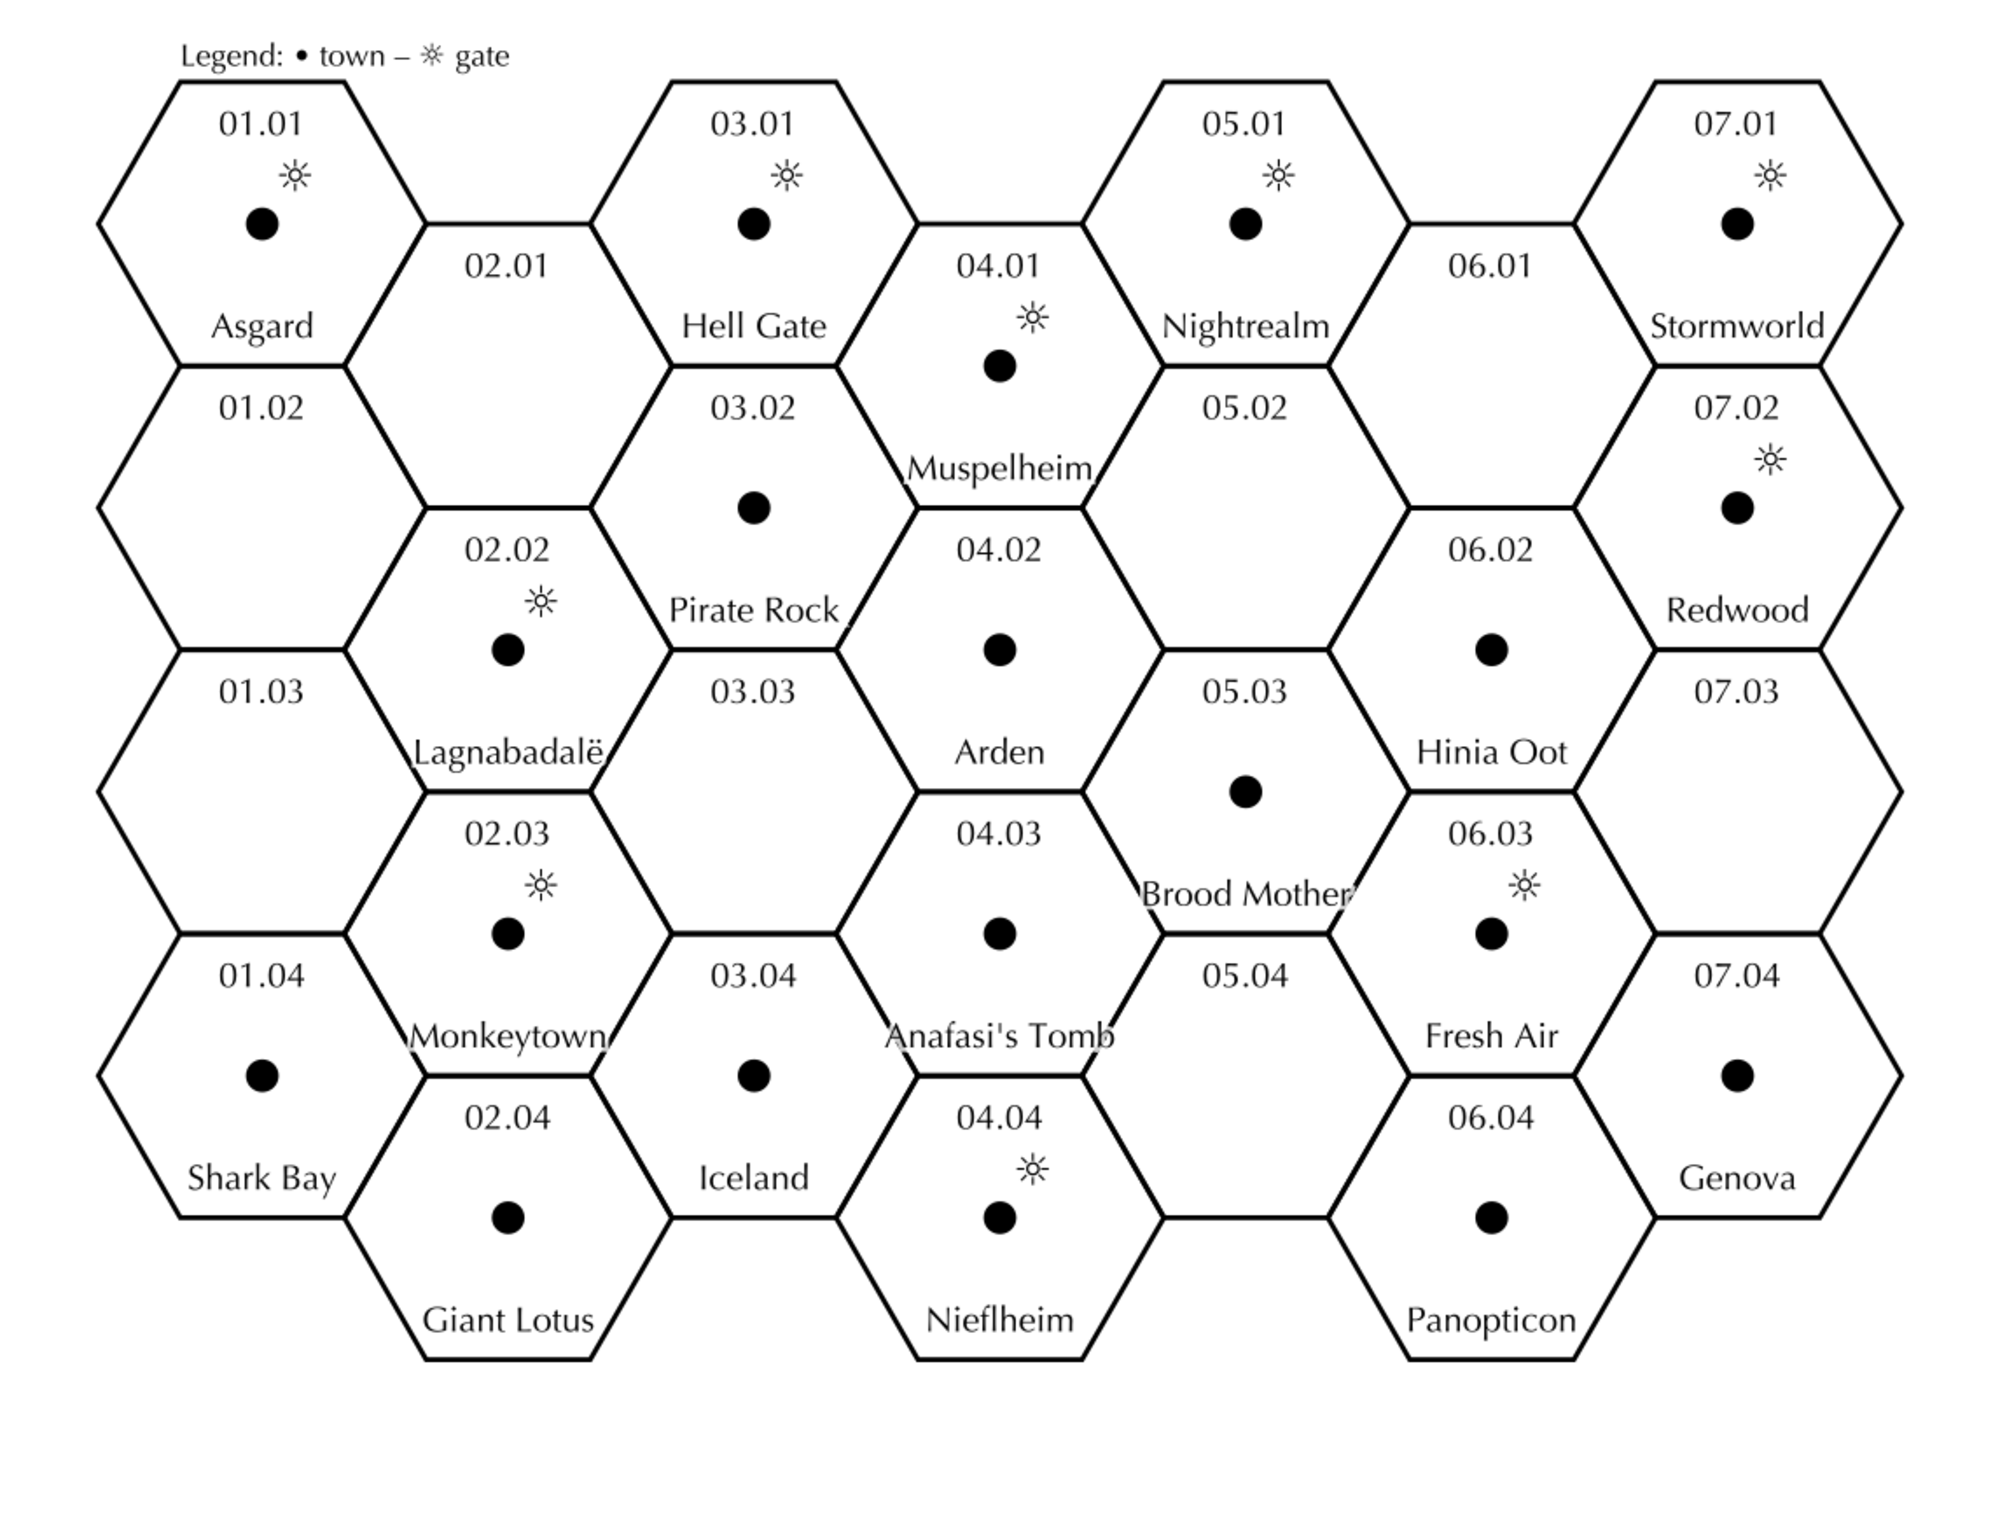
\includegraphics[width=15cm]{Astral-Sea.png}
\end{figure*}

\subsection{Rumors}

\begin{itemize}
\item Asteroids fly through the darkness, their caverns and craters filled with vampires and ghouls
\item There are islands bearing life floating in the Astral Sea
\item All life clings to \textit{portals} of one sort or another
\item Perhaps light and warmth spills over from a plane of eternal fire such as Muspelheim, or from glowing plants or stones
\item There are people who can summon and control \textit{astral whales} and \textit{sky squids}
\end{itemize}

\subsection{Encounters}

With a flying ship, travel from one hex to the next takes about a day. There's a 1 in 6 chance per day of random ship encounters. Roll 1d6:

\begin{enumerate}
\item monkeyman caravel
\item squidman nautilus
\item eelman centipede
\item vampire deathrock 
\item void pirate pike
\item sharkman hammer
\end{enumerate}

If there is no random encounter, there are still harmless natural encounters. Roll 1d4:

\begin{enumerate}
\item astral whales
\item sky squids
\item asteroid field
\item rainbow nebula
\end{enumerate}

\subsection{Ship Combat}

The \textit{Labyrinth Lord} rules cover ship combat. The \textit{Spelljammer} rules have even more ship combat rules. Here's a simple alternative. Ships have hit points and armor class. When a \textbf{catapult} is manned by 4 crew, it takes four rounds to reload (\textit{rate of fire} is 5), it attacks as a fighter level 4 and it does 3d6 damage. Use one roll to attack the ship and a target person visible on deck, if any. If the roll hits, apply damage. If there is a second target person nearby, it is automatically targeted as well.

When a ship is brought to zero hit points and every time it is hit thereafter it takes critical damage. Roll 1d8:

\begin{enumerate}
\item spectacular explosion, all is gone, everybody takes an extra 5d6
\item slow motion breaking up of the ship, everything is gone but the crew is unharmed
\item ship breaks into several pieces, everything is broken but lifeboats or the like can be fixed an hour
\item a disabling hit, immobilizing the ship, all infrastructure breaks down, no more catapult use
\item fire breaks out and spreads unless five crew deal with it for half an hour
\item a gaping hole in the hull immobilizes the ship and provides a extra ingress for boarders
\item a crippling shot immobilizes the ship, taking down mast and rigging, destroying oars and the like
\item the hit reduces the ship's speed as a mast, sail or some oars are taken out; no fleeing from the scene
\end{enumerate}

\textbf{When a ship tries to run}, roll 2d6, +1 if the fleeing ship is significantly smaller than the pursuing ship. On a 10+, you get away because of some lucky shots discouraging your enemies, or because you dove into an asteroid field, or because you managed to make it into a nebula. On a 7--9, you get away but the ship takes damage necessitating a lengthy overhaul in a shipyard. Perhaps you smashed into some asteroids or you took a few hits from parting shots. On a 6+, you did not make it. Fight to the bitter end or surrender now.

\subsection{Monkeyman Caravel}

"Monkeymen" is what other people call humans – humanoids with monkey heads. A caravel is a small trading ship made of wood with a single catapult and 10 crew. HP 20 AC 9 3d8.

The prize usually consists of ten tons of pickled lotus flesh, wooden planks, grains and wine barrels, cactus figs, fungus lanterns, or some other produce worth 1d4 × 10,000 gold and the ship itself is worth another 10,000 gold. Clearly, being a pirate is lucrative.

\subsection{Squidman Nautilus}

This is a slaver ship built atop a trained nautilus with two mounted catapults. The crew consists of squidmen, slaves manning two catapults and intelligent giant spiders. The shell provides excellent protection. HP 30 AC 2 3d8/3d8.

The nautilus' ten \textbf{tentacles} are used to pick up victims and deliver them into the slave hold. Each tentacle acts as a separate creature. HD 1 AC 2 1d4 MV 3 ML 10 XP 13; when hit, save vs. poison or be \textit{paralyzed} for 10min.

The five \textbf{squidmen} have terrible psi powers but they are cowards. HD 7+1 AC 8 1d6 F7 MV 12 ML 6 XP 1300; \textit{mind blast} at will stuns anybody in a cone 60ft long unless they save vs. paralysis; \textit{domination} at will forces a single victim to do and say exactly as their new master wish unless they save vs. spells; \textit{read thoughts} lets them read any thoughts within 60ft.

The fifteen \textbf{slaves} are humans manning the catapults and repairing damage. HD 1 AC 9 1d6 F1 MV 12 ML 6 XP 10.

The ten \textbf{giant spiders} trained to paralyze victims and drag them back to their masters. HD 4+1 AC 5 1d8 F2 MV 12 ML 8 XP 215; when bitten, save vs. paralysis or drop into a death-like trance for 6h; they can jump for 20ft and get +1 to hit when they do. They speak of hunting and feeding.

There is a 1 in 6 chance that this slaver ship is actually on the way back to Hinia Oot and its hold is filled with fifty \textbf{slaves}. As these would be sold for 25,000 gold, freeing them would be worth as many XP. The ship itself is worth 35,000 gold.

\end{document}
